
\FloatBarrier

\section{Система Ван-дер-Поля} %  % {{{1 _VDP_
\label{atu:sect:vdp}

\LinkRef{
  vdp: ASAU-16, 17(alt), ITMM-2011
}

\subsection{Определение системы и анализ её динамики} %  % {{{2 _vdp_task

% TODO: dyn_sys_chaos, chaos_in_phase_dyn_VDP_modul_dobr.pdf buffer_phemon_vdp

Модель нелинейной автоколебательной системы Ван-Дер-Поля~(\ref{atu:eq:vdp})
широко используется при исследовании динамики
колебательных систем, в которых происходит восполнение
энергии системы из внешнего источника~\cite{anisch_nonlin_eff,magni_theory_dyn_chaos,atu_asau16}:
%
\begin{equation}
 \ddot{x} - \varepsilon (1-x^2)  \dot{x} + \Omega_0^2 x  = u(t) .
\label{atu:eq:vdp}
\end{equation}
\noindent
где
\(x(t)\) -- координата колебаний,
\( \varepsilon \) -- параметр, определяющий получение
  энергии системой,
\( \Omega_0 \) -- собственная частота при \( \varepsilon = 0 \),
\(u(t)\) -- внешнее возмущающее воздействие.

При \( \varepsilon > 0 \) и \( u(t) = 0 \)
рассматриваемая система реализует режим автоколебаний
с постоянной частотой, зависящей от \( \varepsilon \):
%
\begin{equation}
\Omega \approx \Omega_0 \sqrt{ 1 - \left( \frac{\varepsilon}{2 \Omega_0} \right)^2 }.
\label{atu:eq:vdp_Omega}
\end{equation}

При этом амплитуда колебаний остаётся практически постоянной,
а сама форма колебаний принимает всё более нелинейный характер.

Под воздействием входного гармонического сигнала
\( u(t) = U_{in} \sin ( \omega_{in} t ) \)
система~(\ref{atu:eq:vdp}) может проявлять регулярную, сложно-периодическую
и хаотическую динамику.

Идентифицируемый параметр \( \varepsilon \)
характеризует поступление энергии в систему.
При $x \approx 0$ членом с $x^2$ можно пренебречь,
и нелинейность вырождается в ``отрицательное трение''.
При больших амплитудах колебаний член с $x^2$
начинает преобладать, там самым ограничивая рост амплитуды.

При анализе численного моделирования системы~(\ref{atu:eq:vdp})
следует осторожно относится к выводам о типе динамики,
которые можно сделать, исходя из фазового или расширенного фазового портрета.
Например, на рис.~\ref{atu:f:vdp_phase_f_reg},
при условиях
$ \varepsilon=1.50$, $U_{in}=0.3$, $\omega_{in}=0.27$
на левом графике
фазовая траектория получается плотной,
однако спектр свидетельствует о регулярной динамике
с ограниченным набором частот.

\begin{figure}[ht!]
\begin{center}
  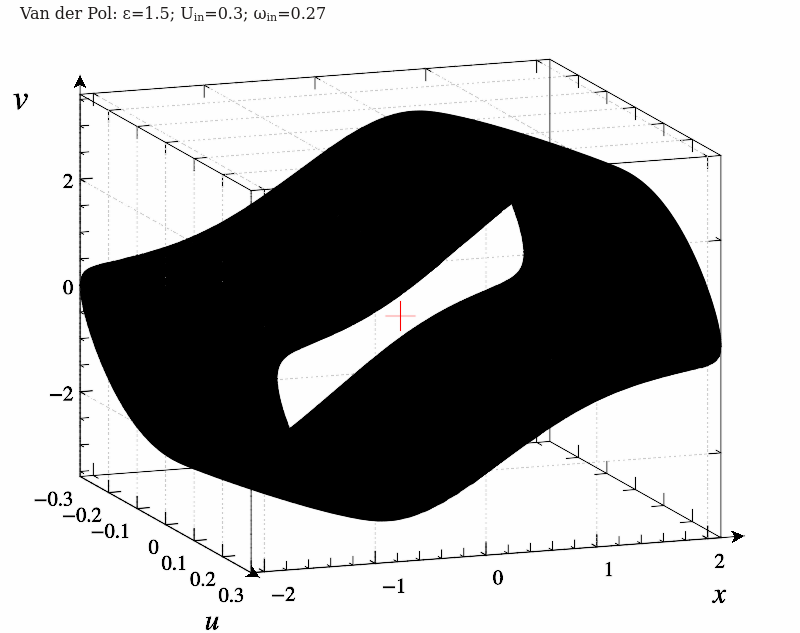
\includegraphics[width=0.49\textwidth]{p/cha/vdp/vdp_0-p_ph2d_1x50_0x30_0x27.png}
  \hfill
  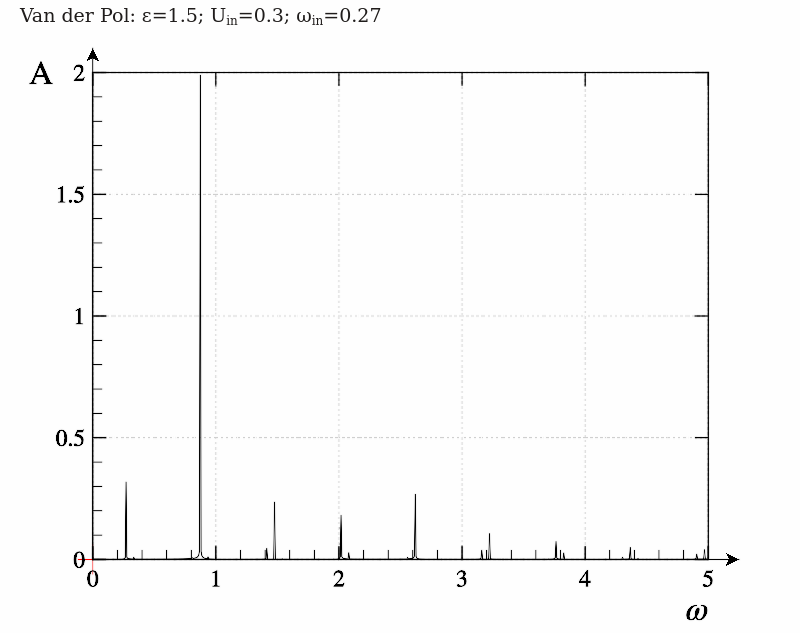
\includegraphics[width=0.49\textwidth]{p/cha/vdp/vdp_fft-p_f_1x50_0x30_0x27.png}
\end{center}
  \caption{Расширенный фазовый портрет и спектр системы Ван-дер-Поля (\ref{atu:eq:vdp}) в режиме регулярных колебаний}
\label{atu:f:vdp_phase_f_reg}
\end{figure}

Непосредственно хаотические колебания этой системы часто характеризуются
менее выраженной плотностью аттрактора. Тем не менее,
участки сложного спектра (рис.~\ref{atu:f:vdp_phase_f_chaos})
свидетельствуют в пользу хаоса.
Данная иллюстрация соответствует условиям
$ \varepsilon=2.65$, $U_{in}=1.2$, $\omega_{in}=0.27$.
При этом малые изменения параметров, например
снижение величины $\varepsilon$ до $2.5$
приводит к реализации режима простых регулярных колебаний.

\begin{figure}[ht!]
\begin{center}
  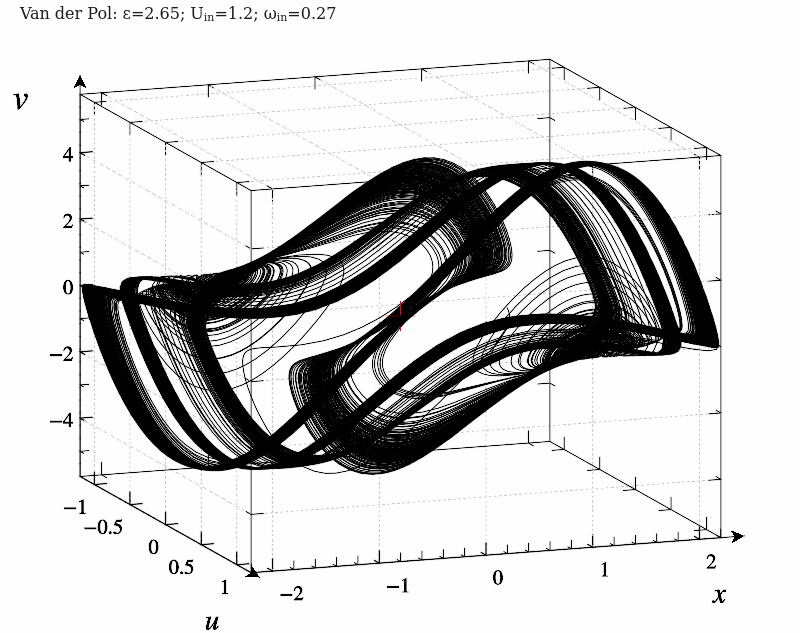
\includegraphics[width=0.49\textwidth]{p/cha/vdp/vdp_0-p_ph2d_2x65_1x20_0x27.png}
  \hfill
  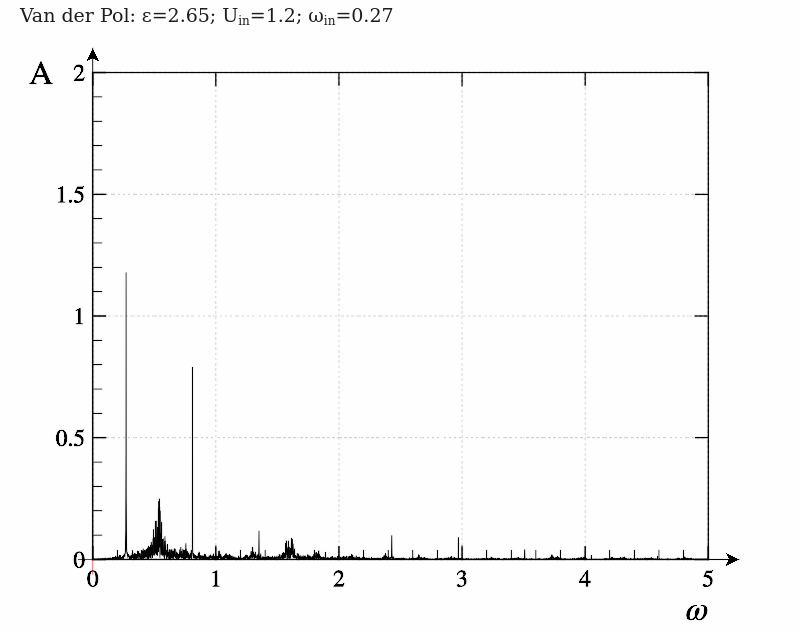
\includegraphics[width=0.49\textwidth]{p/cha/vdp/vdp_fft-p_f_2x65_1x20_0x27.png}
\end{center}
  \caption{Расширенный фазовый портрет и спектр системы Ван-дер-Поля (\ref{atu:eq:vdp}) в режиме хаотических колебаний}
\label{atu:f:vdp_phase_f_chaos}
\end{figure}

Анализ спектра системы Ван-дер-Поля, как и многих других систем
динамического хаоса, следует проводить, учитывая
спектральное разрешение.
Например, на  рис.~\ref{atu:f:vdp_phase_f_complex}
представлены результаты моделирования системы при
$ \varepsilon=4.8$, $U_{in}=0.7$, $\omega_{in}=0.7$.
В спектре системы наблюдаются участки с очень близко
расположенными пиками. При недостаточной разрешающей способности
этот участок будет принят за зону сплошного спектра.
Это может привести к выводу о хаотичности системы,
тем более, если учесть вид аттрактора.

\begin{figure}[ht!]
\begin{center}
  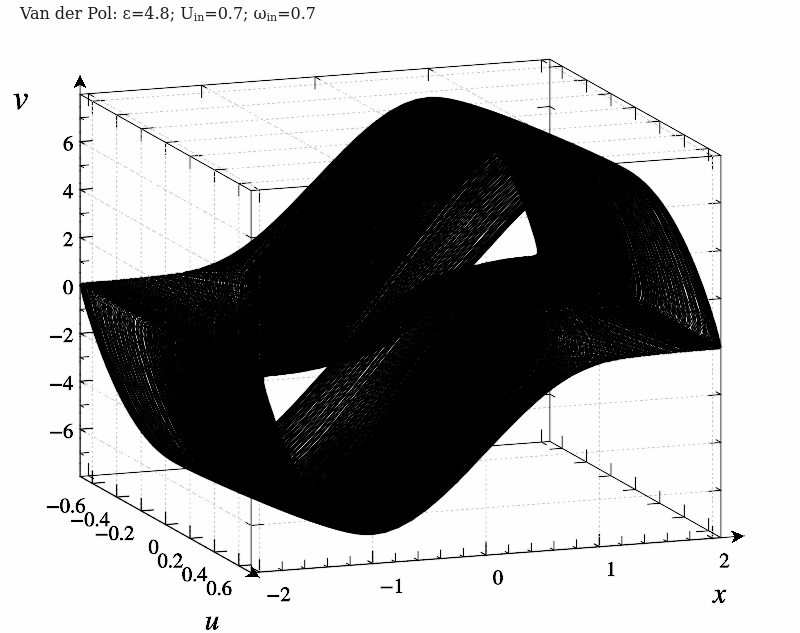
\includegraphics[width=0.49\textwidth]{p/cha/vdp/vdp_0-p_ph2d_4x80_0x70_0x70.png}
  \hfill
  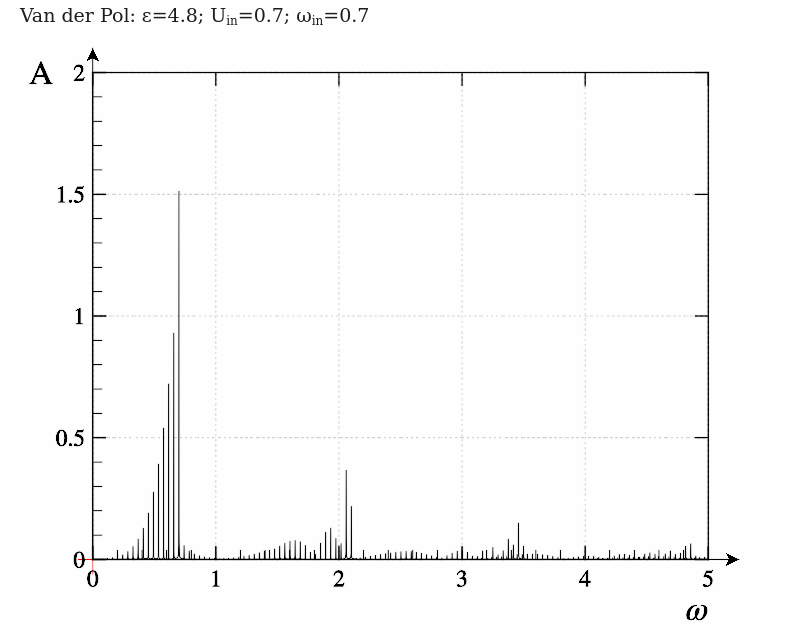
\includegraphics[width=0.49\textwidth]{p/cha/vdp/vdp_fft-p_f_4x80_0x70_0x70.png}
\end{center}
  \caption{Расширенный фазовый портрет и спектр системы Ван-дер-Поля (\ref{atu:eq:vdp}) в режиме сложных регулярных колебаний}
\label{atu:f:vdp_phase_f_complex}
\end{figure}


% \begin{figure}[htb!]
% \centerline{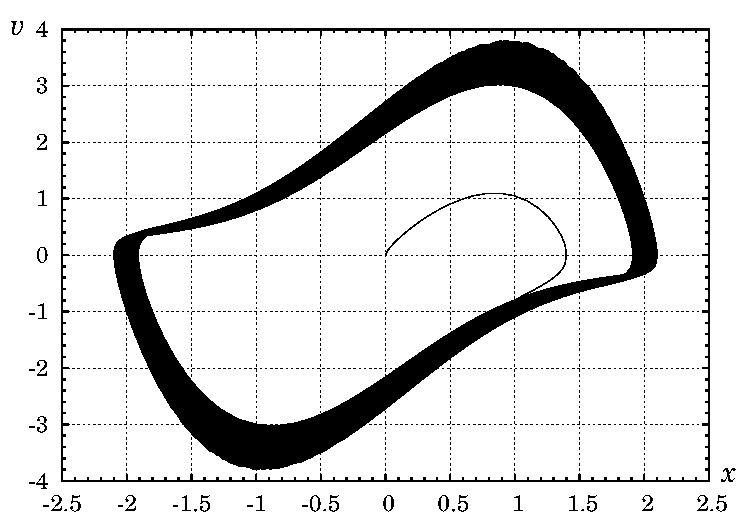
\includegraphics[width=0.5\textwidth]{p/cha/vdp_phase.pdf} }
% \caption{Фазовый портрет системы Ван-дер-Поля (\ref{atu:eq:vdp})}
% \label{atu:f:vdp_phase}
% \end{figure}

При анализе физических систем нет возможности произвольным образом
задавать время измерения для получения спектра с требуемым разрешением.
Более того, с учётом ограниченной точности измерений нет возможности
точно определить показатели Ляпунова. Таким образом,
вполне возможно существование систем, неотличимых от хаотических
при проведении измерений, но не являющимися хаотическими в строгом понимании.
Тем не менее, с точки зрения задачи идентификации,
этот случай практически неотличим от реального хаоса, и требует
применения соответствующих методов и критериев.

% }}}2


\subsection{Анализ и выбор критериев}  % {{{2

В отличие от систем Лоренца, Рёсслера и им подобных,
у системы Ван-дер-Поля есть только одна наблюдаемая величина: $x$.
Это сразу сильно ограничивает круг критериев, требующих анализа.

На первый взгляд, если доступен сигнал $x(t)$,
то можно вычислить сигналы $\dot{x}(t)$ и $\ddot{x}(t)$.
После этого, подставив получившиеся зависимости в (\ref{atu:eq:vdp}),
можно получить значение идентифицируемого параметра.
На самом деле, это возможно только в случае практически полного отсутствия помех.
Даже небольшой  (0.001\%) уровень ошибок измерения
при вычислении производных, особенно второй,
приводит к совершенно произвольным результатам.
Таким образом, и для этой системы без применения
интегральных критериев нет возможности создать работоспособную систему идентификации.

Критерии $q_{x^2}$, $q_{rx}$ и $q_{|x|}$ отличаются
для этой задачи непринципиально.
Несмотря на то, что эти величины в данном конкретном случае не
отображают какой-либо закон сохранения, их применение может быть оправданным~\cite{atu_asau17}.
При росте параметра $\varepsilon$ система всё больше проявляет нелинейные свойства.
Это выражается в том, что при одинаковой амплитуде сигнала
зависимость $x(t)$ большую часть времени проводит вблизи
амплитудных значений, что приводит к росту этих критериев.
Для определённости в дальнейшем будем использовать $q_{x^2}$.

Также имеет смысл рассмотреть достаточно очевидный для
колебательных систем критерий $q_T$,
заключающийся в измерении ``периода''~\cite{atu_asau16}.
Очевидно, что понятие периода для хаотических систем неприменимо.
Однако, можно принять за текущее значение периода
интервал времени между двумя последовательными срабатываниями
правильно настроенного триггера Шмидта, на вход которого подаётся сигнал
$x(t)$. Этот подход используется при построении входных
цепей частотомеров. При этом автоматически происходит усреднение
на интервалах порядка этого ``периода''. Однако,
для систем идентификации такое усреднение скорее всего будет
недостаточным, особенно в хаотических и сложно-периодических
режимах. Следовательно, имеет смысл использовать дополнительное
усреднение, например~(\ref{atu:eq:qlin}).

Рассмотрим характерные зависимости рассматриваемых критериев,
полученные в результате моделирования динамики системы (\ref{atu:eq:vdp}).
На  рис.~\ref{atu:f:vdp_q1} представлен вид этих зависимостей
для различных условий.


\begin{figure}[ht!]
\begin{center}
  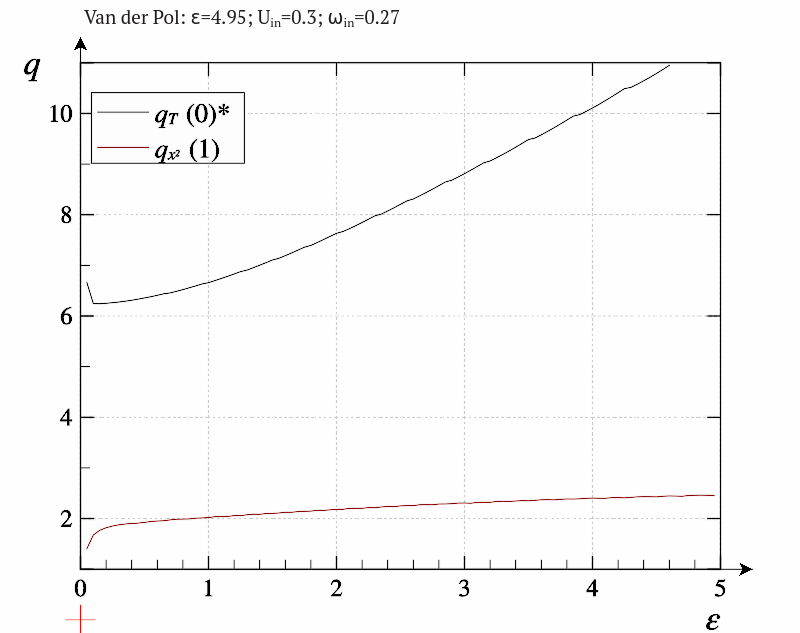
\includegraphics[width=0.49\textwidth]{p/cha/vdp/vdp_q-p_q_0x30_0x27.png}
  \hfill
  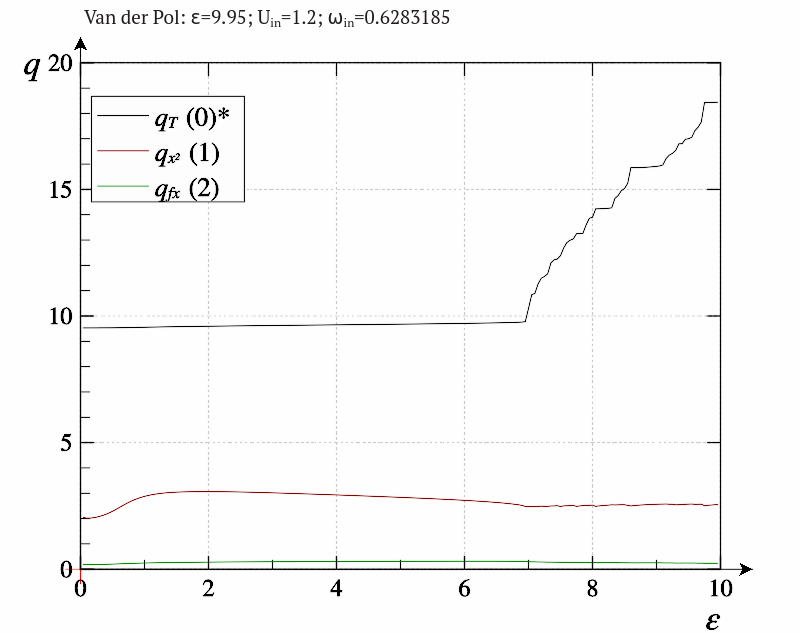
\includegraphics[width=0.49\textwidth]{p/cha/vdp/vdp_q-p_q_1x20_0x6283185.png}
\end{center}
  \caption{Зависимости $q_{x^2}(\varepsilon)$ и $q_T(\varepsilon) $ системы Ван-дер-Поля}
\label{atu:f:vdp_q1}
\end{figure}

Левый график соответствует такому набору параметров,
при котором наблюдается периодическое и сложно-периодическое движение.
При этом оба критерия подходят для синтеза системы идентификации, а
критерий $q_T$ проявляет меньшую нелинейность.
Правый график отображает случай, когда изменение параметра $\varepsilon$
приводит к существенному изменению поведения.
При $\varepsilon < 7 $ происходит ``захват частоты'',
то есть возмущающий сигнал $u(t)$ ``навязывает'' свою частоту системе,
что приводит к простой динамике и отсутствию зависимости $q_T$ от $\varepsilon$.
Идентификация на данном участке невозможна, ввиду
отсутствия влияния параметра на ``период''.
Правая часть этого графика отображает постоянные переходы от
сложных колебаний к хаосу и обратно. На зависимости $q_T(\varepsilon)$
появляются изломы, что потенциально должно привести к снижению
точности идентификации на фоне общей работоспособности.
График зависимости $q_{x^2}(\varepsilon)$ имеет экстремальный характер,
что позволяет использовать этот критерий только на тех диапазонах $\varepsilon$,
на которых наблюдается монотонность.

Рассмотрим зависимости $q_T(\varepsilon,U_{in})$ и $q_{x^2}(\varepsilon,U_{in})$
для различных значений $\omega_{in}$.
На  рис.~\ref{atu:f:vdp_q2_027}
представлены эти зависимости при $\omega_{in}=0.27$.


\begin{figure}[ht!]
\begin{center}
  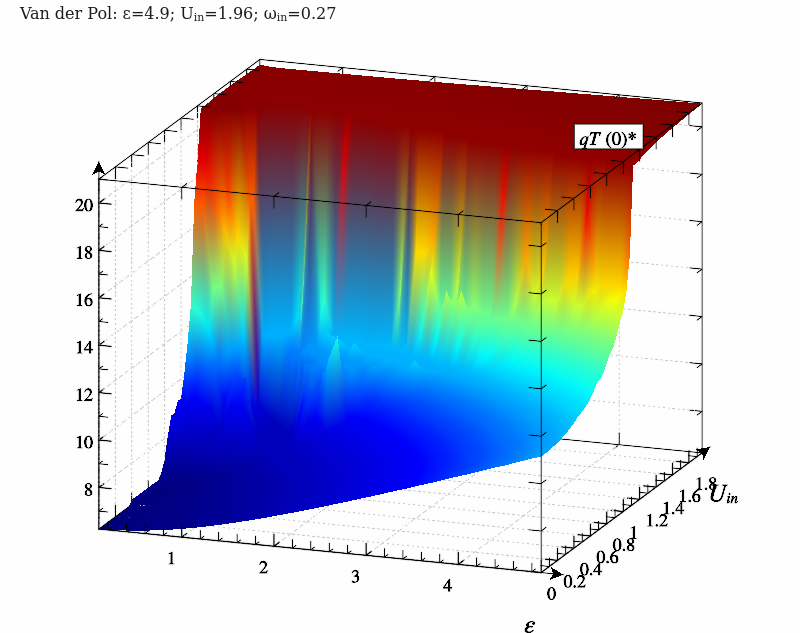
\includegraphics[width=0.49\textwidth]{p/cha/vdp/vdp_q_2d-p_qT_ome_0x27.png}
  \hfill
  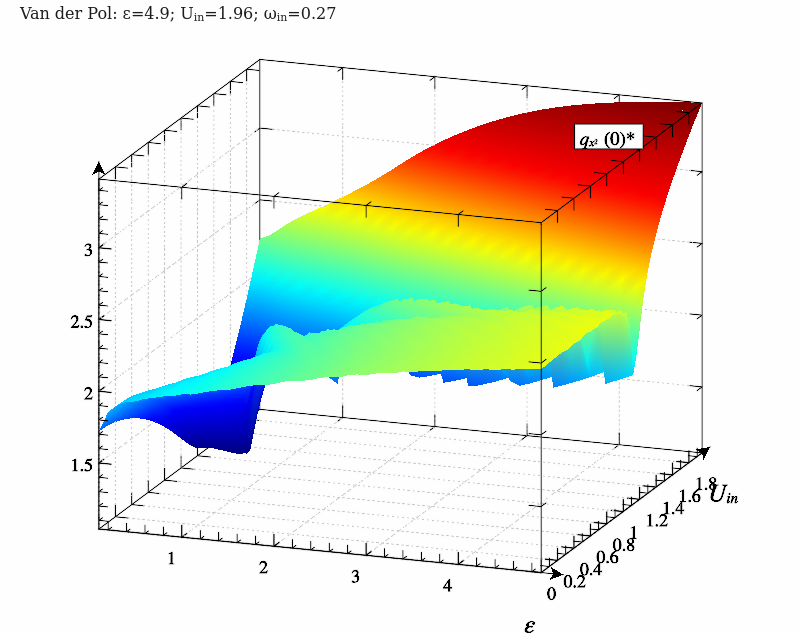
\includegraphics[width=0.49\textwidth]{p/cha/vdp/vdp_q_2d-p_qx2_ome_0x27.png}
\end{center}
  \caption{Зависимости $q_T(\varepsilon,U_{in})$ и $q_{x^2}(\varepsilon,U_{in})$  при $\omega_{in}=0.27$}
\label{atu:f:vdp_q2_027}
\end{figure}

При высоких значениях $U_{in}$ происходит захват частоты,
график зависимости $q_T(\varepsilon,U_{in})$ в этой области
представляет собой плоскую поверхность, что свидетельствует
о неприменимости критерия в этих условиях. При малых значения $U_{in}$,
наоборот, наблюдается достаточно близкая к линейной зависимость.
В промежутке между двумя этими областями возможности
идентификации с использованием данного критерия существуют, но ограничены.
Критерий $q_{x^2}$ при этих же условиях имеет несколько другие ограничения.
Идентификация затруднена в области ``оврага'', который соответствует
переходному режиму на предыдущем графике.
Как в области низких, так и в области высоких значений
$U_{in}$ идентификация возможна.

На  рис.~\ref{atu:f:vdp_q2_120}
представлены поверхности критериев при $\omega_{in}=1.2$.

\begin{figure}[ht!]
\begin{center}
  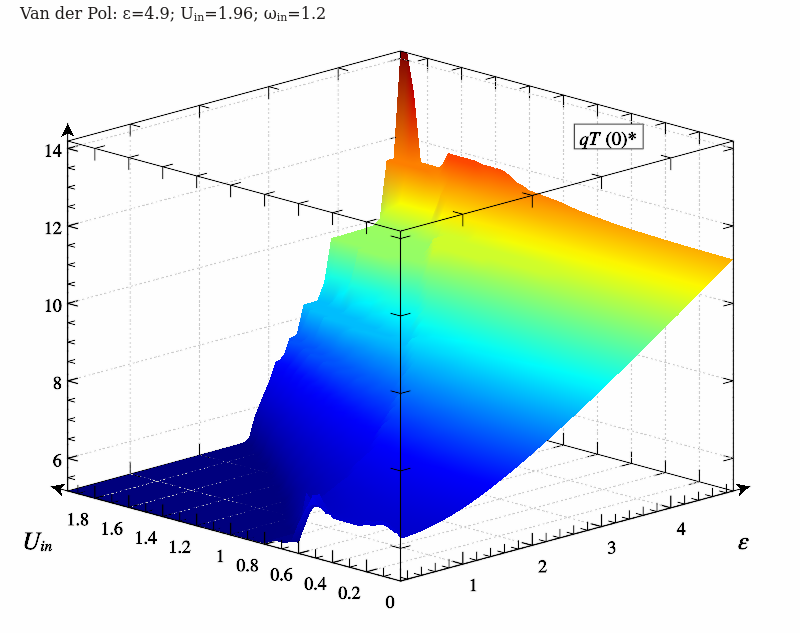
\includegraphics[width=0.49\textwidth]{p/cha/vdp/vdp_q_2d-p_qT_ome_1x20.png}
  \hfill
  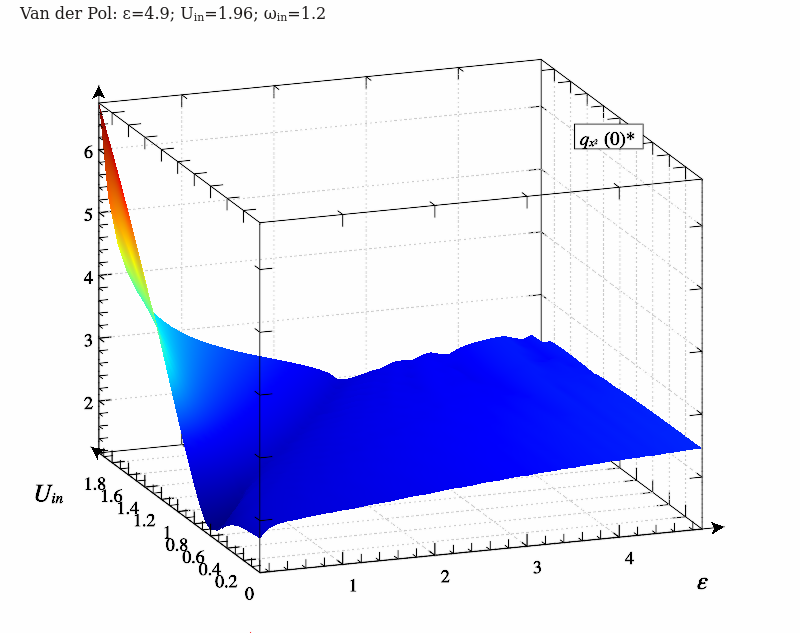
\includegraphics[width=0.49\textwidth]{p/cha/vdp/vdp_q_2d-p_qx2_ome_1x20.png}
\end{center}
  \caption{Зависимости $q_T(\varepsilon,U_{in})$ и $q_{x^2}(\varepsilon,U_{in})$  при $\omega_{in}=1.2$}
\label{atu:f:vdp_q2_120}
\end{figure}

На зависимости $q_T(\varepsilon,U_{in})$ в этом случае также виден
плоский участок, соответствующий режиму захвата частоты.
Но большая часть этой зависимости свидетельствует о том, что
идентификация возможна, и при этом скорее всего
будет наблюдаться увеличение ошибки идентификации из-за неравномерности графика.
Напротив, зависимость $q_T(\varepsilon,U_{in})$ проявляет
мультимодальный характер, что позволяет проводить идентификацию только в узких диапазонах.

Таким образом, установлено, что ни один из рассматриваемых критериев не
обеспечивает возможность идентификации при любых значениях параметров.
Однако, наибольший диапазон работоспособности продемонстрировал критерий $q_{T}$.
Он и будет использован в дальнейших исследованиях. При этом при постановке задачи
будем избегать режимов, на которых происходит захват частоты.









% }}}2

\subsection{Тестовая задача идентификации для системы Ван-дер-Поля}  % {{{2

При синтеза системы идентификации использовалась группа методов ``ql3rlWvnAAW''.
С учётом выбора критерия $q_{T}$ при постановке задачи идентификации
параметры выбирались с учётом диапазона работоспособности этого критерия.
Первая группа значений параметров: $U_{in}=0.3$, $\omega_{in}=0.27$, $ \varepsilon \in [1, 4 ]$.

Рассмотрим процесс идентификации
в квазистационарном случае,
при медленном изменении параметра~(\ref{atu:eq:po_t_ramp}), $p_0=1$, $U_p=2$.
Динамика агентов и различных способов задания $p_\mathrm{id}$
представлена на рис.~\ref{atu:f:vdp_id1_ramp}.

\begin{figure}[ht!]
\begin{center}
  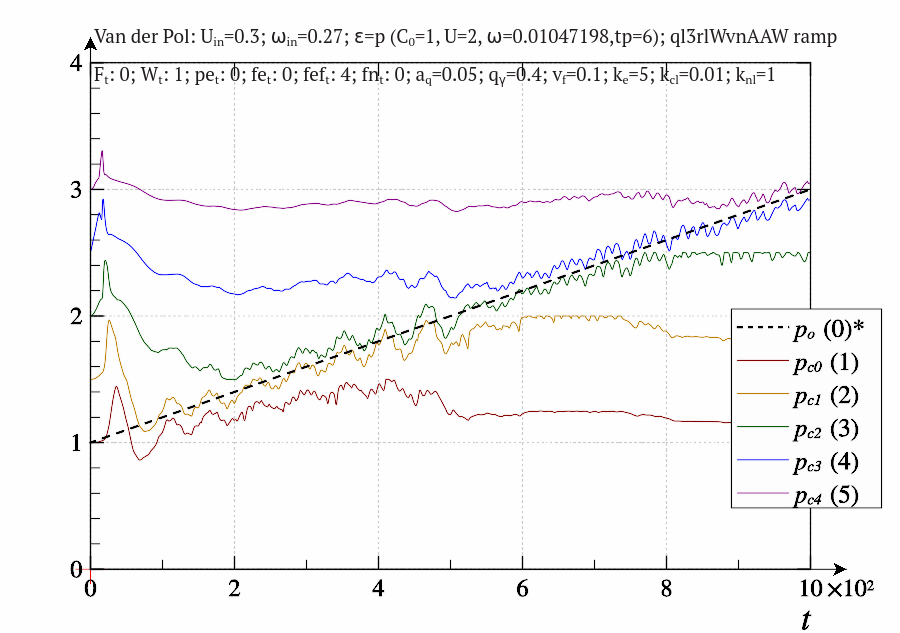
\includegraphics[width=0.49\textwidth]{p/cha/vdp/vdp_id-p_t_pi_ql3rlWvnAAW_ramp.png}
  \hfill
  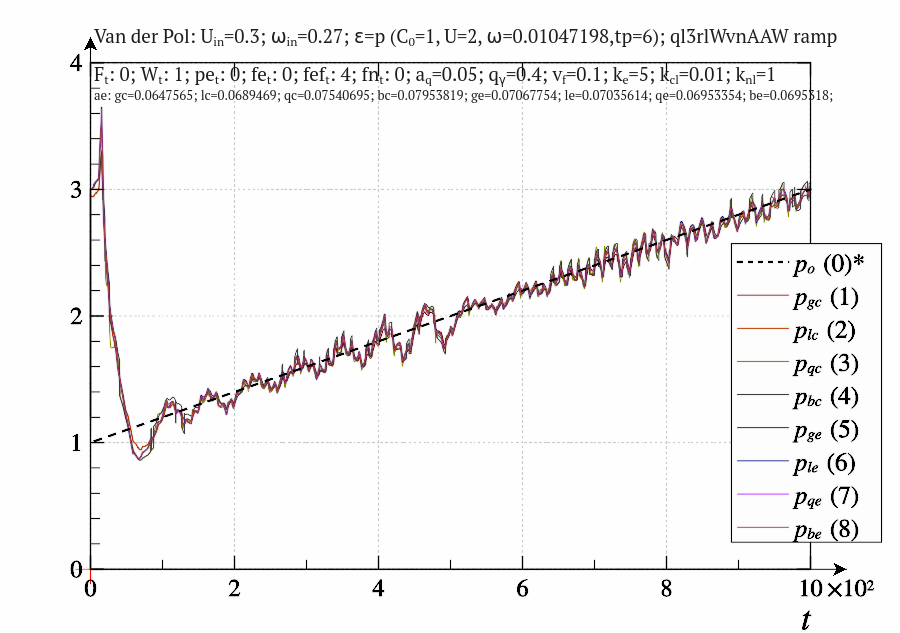
\includegraphics[width=0.49\textwidth]{p/cha/vdp/vdp_id-p_t_p_ql3rlWvnAAW_ramp.png}
\end{center}
  \caption{Динамика агентов и идентифицируемого значения для системы Ван-дер-Поля при условии (\ref{atu:eq:po_t_ramp})}
\label{atu:f:vdp_id1_ramp}
\end{figure}

За исключением начального участка, на котором происходит стабилизация
состояния самой системы идентификации, агенты демонстрируют корректное поведение,
сопровождая медленно изменяющиеся значение параметра $\varepsilon$.
Как следствие, все методы определения $p_\mathrm{id}$
позволяют достаточно точно провести идентификацию.
Небольшие колебания обусловлены тем, что на самом деле
система не в полной мере может быть названа квазистационарной,
из-за большого времени усреднения критерия.
Участков, на которых нарушался бы процесс идентификации,
или же существенно росла ошибка, не наблюдается.

Рассмотрим динамку процесса идентификации
(рис.~\ref{atu:f:vdp_id1_sign})
при условиях (\ref{atu:eq:po_t_sign}), $p_0=2$, $U_p=0.8$, $\omega_{in}=0.01047$.

\begin{figure}[ht!]
\begin{center}
  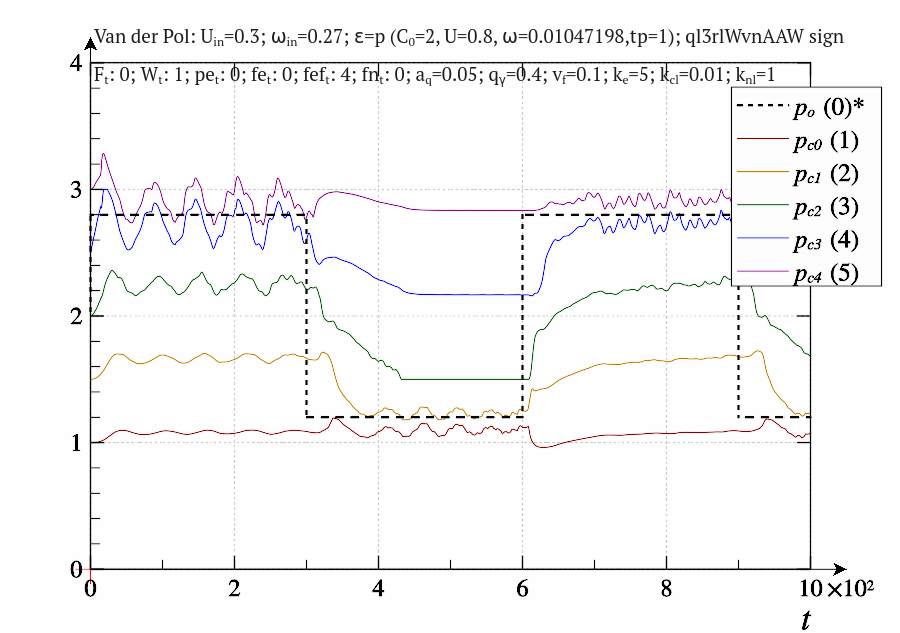
\includegraphics[width=0.49\textwidth]{p/cha/vdp/vdp_id-p_t_pi_ql3rlWvnAAW_sign.png}
  \hfill
  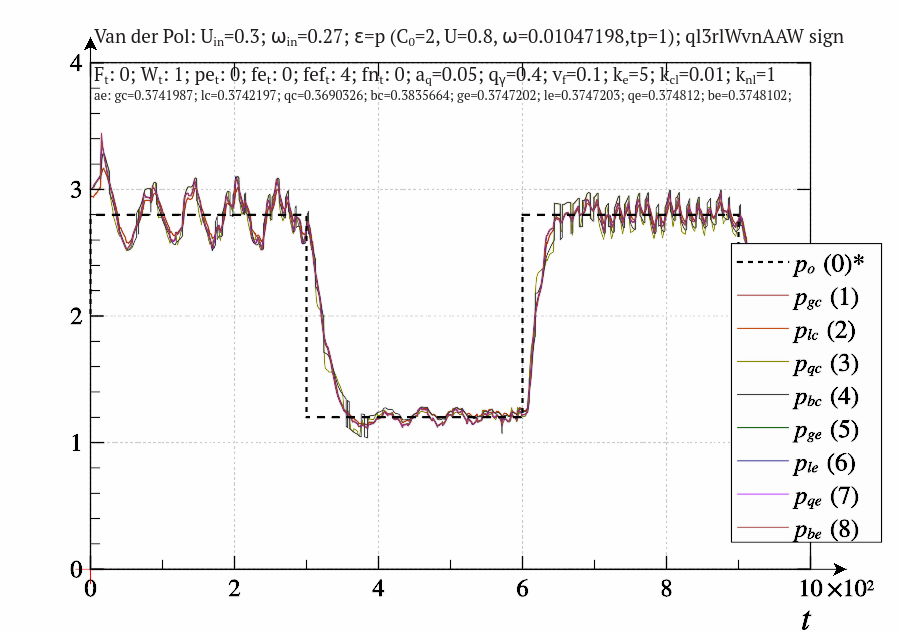
\includegraphics[width=0.49\textwidth]{p/cha/vdp/vdp_id-p_t_p_ql3rlWvnAAW_sign.png}
\end{center}
  \caption{Динамика агентов и идентифицируемого значения для системы Ван-дер-Поля при условии (\ref{atu:eq:po_t_sign})}
\label{atu:f:vdp_id1_sign}
\end{figure}

Как уже наблюдалось, все методы определения $p_\mathrm{id}$
на уровне координатора поиска дают схожие результаты.
Следует отметить заметные колебания на первой половине периода изменения
параметра, по сравнению с третей. Избыточные колебания на начальном этапе можно
уменьшить путём предварительной настройки элементов усреднения критерия.
Однако, для такой настройки необходима дополнительная информация,
которая неизвестна a priori.

На рис.~\ref{atu:f:vdp_id1_sin}
представлены аналогичные результаты,
но в случае плавного изменения параметра~(\ref{atu:eq:po_t_sin}).

\begin{figure}[ht!]
\begin{center}
  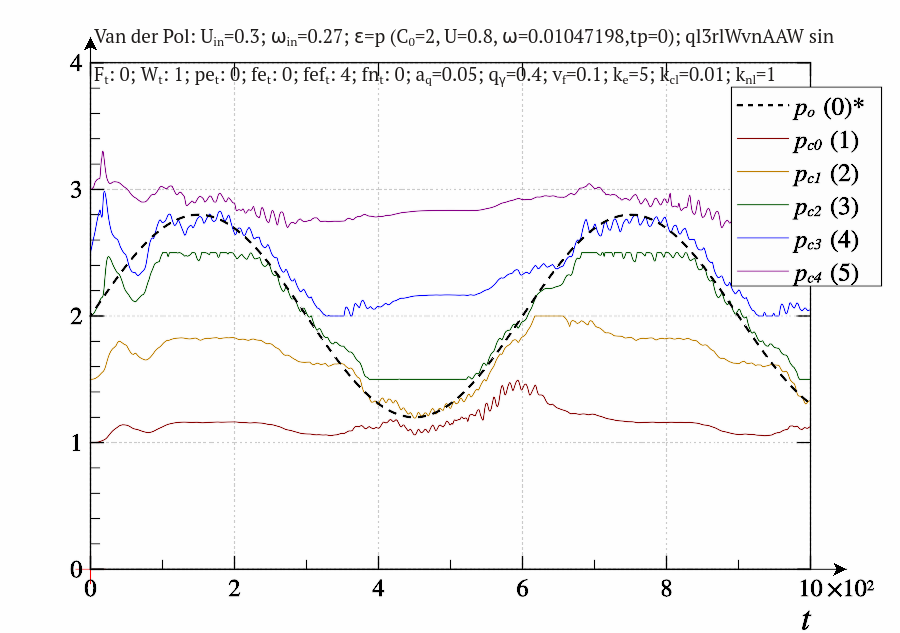
\includegraphics[width=0.49\textwidth]{p/cha/vdp/vdp_id-p_t_pi_ql3rlWvnAAW_sin.png}
  \hfill
  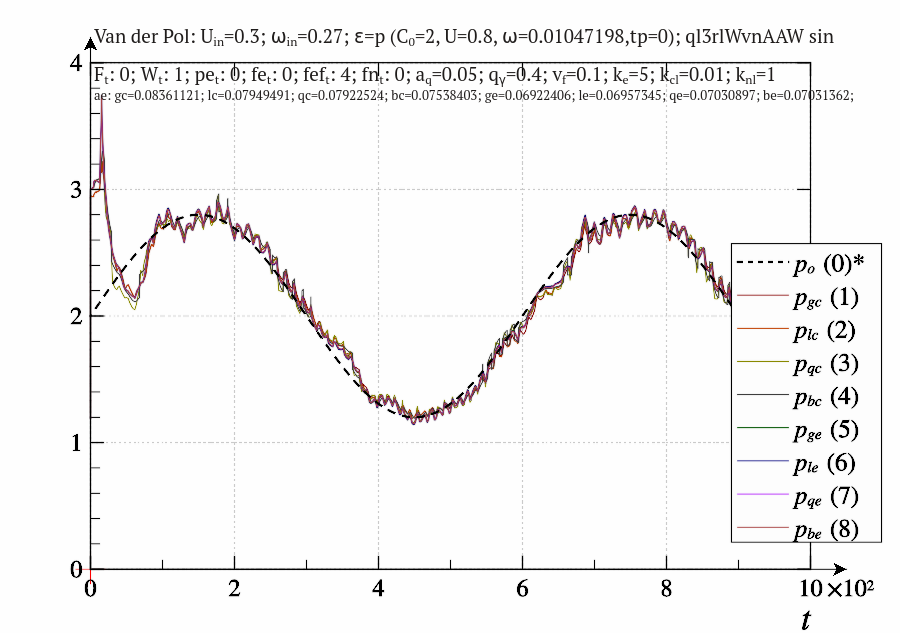
\includegraphics[width=0.49\textwidth]{p/cha/vdp/vdp_id-p_t_p_ql3rlWvnAAW_sin.png}
\end{center}
  \caption{Динамика агентов и идентифицируемого значения для системы Ван-дер-Поля при условии (\ref{atu:eq:po_t_sin})}
\label{atu:f:vdp_id1_sin}
\end{figure}

Ошибка идентификации в этом случае существенно меньше, при сохраняющихся
колебаниях на начальном этапе.

% }}}2


\subsection{Влияние параметров системы идентификации на ошибку идентификации для системы Ван-дер-Поля}  % {{{2

При идентификации системы Ван-дер-Поля
с использованием критерия $q_T$
влияние параметра $a_q$ представляет
особый интерес, ввиду наличия двух уровней усреднения.
Зависимости усреднённых ошибок идентификации
от этого параметра представлены на  рис.~\ref{atu:f:vdp_e_a_q}.

\begin{figure}[ht!]
\begin{center}
  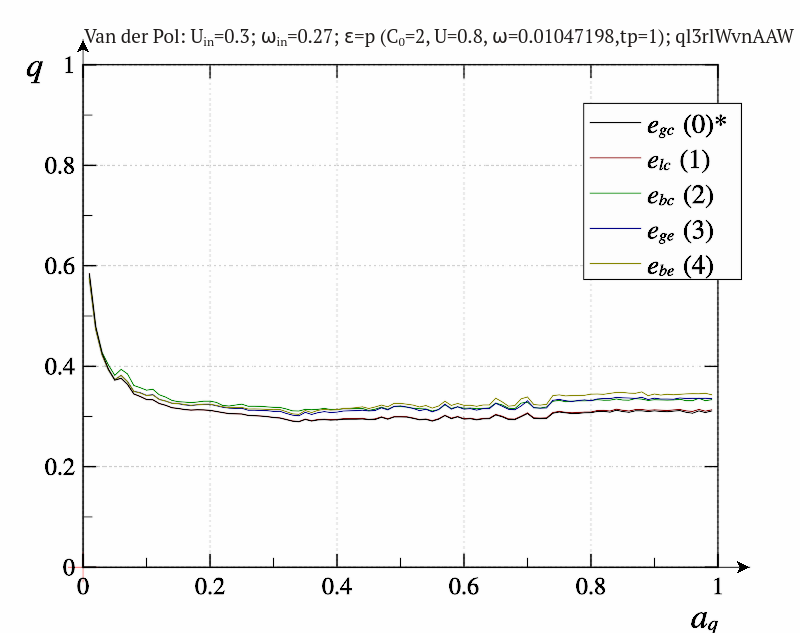
\includegraphics[width=0.49\textwidth]{p/cha/vdp/vdp_id-p_a_q_sign.png}
  \hfill
  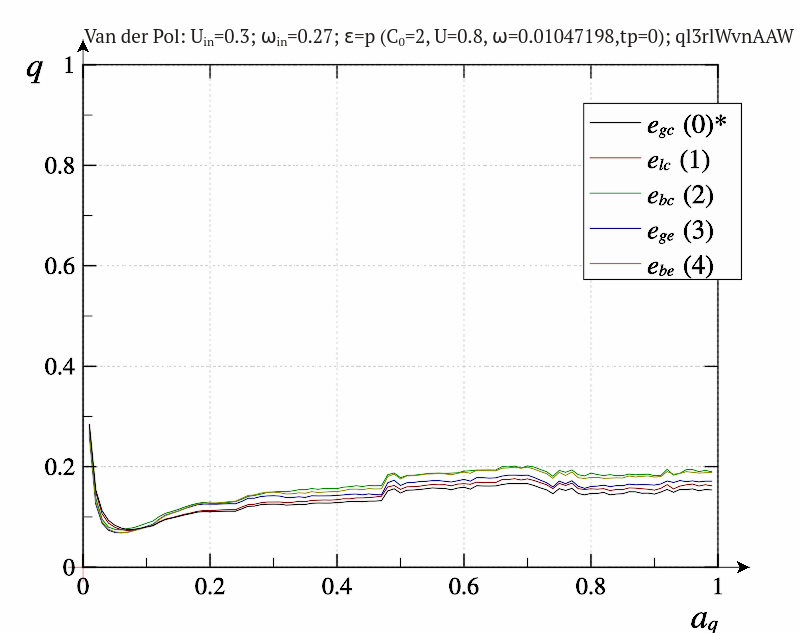
\includegraphics[width=0.49\textwidth]{p/cha/vdp/vdp_id-p_a_q_sin.png}
\end{center}
  \caption{Зависимости $\bar{e}(a_q)$ для системы Ван-дер-Поля}
\label{atu:f:vdp_e_a_q}
\end{figure}

Исходя из характерных значений ``периода'' можно было ожидать
изменение характера этих зависимостей при $a_q \approx 0.1$.
Однако, никаких существенных изменений на графиках не обнаружено.
Сам вид этих зависимостей практически ничем, кроме масштаба,
не отличается от таковых для уже рассмотренных систем.
Таким образом получил подтверждение тезис о необходимости
дополнительного усреднения на этом этапе.

Рассмотрим влияние ещё одного параметра системы идентификации --- $q_\gamma$.
Соответствующие зависимости приведены на  рис.~\ref{atu:f:vdp_e_q_gamma}.

\begin{figure}[ht!]
\begin{center}
  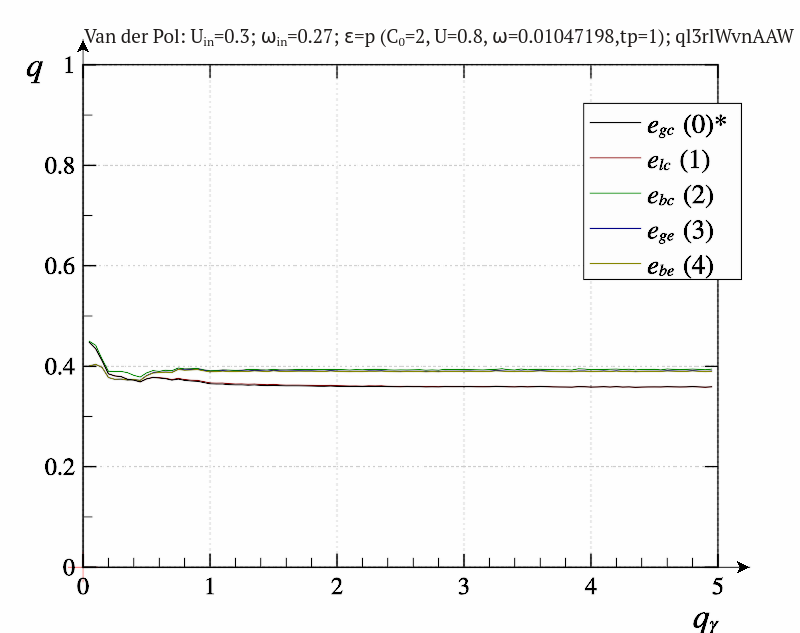
\includegraphics[width=0.49\textwidth]{p/cha/vdp/vdp_id-p_q_gamma_sign.png}
  \hfill
  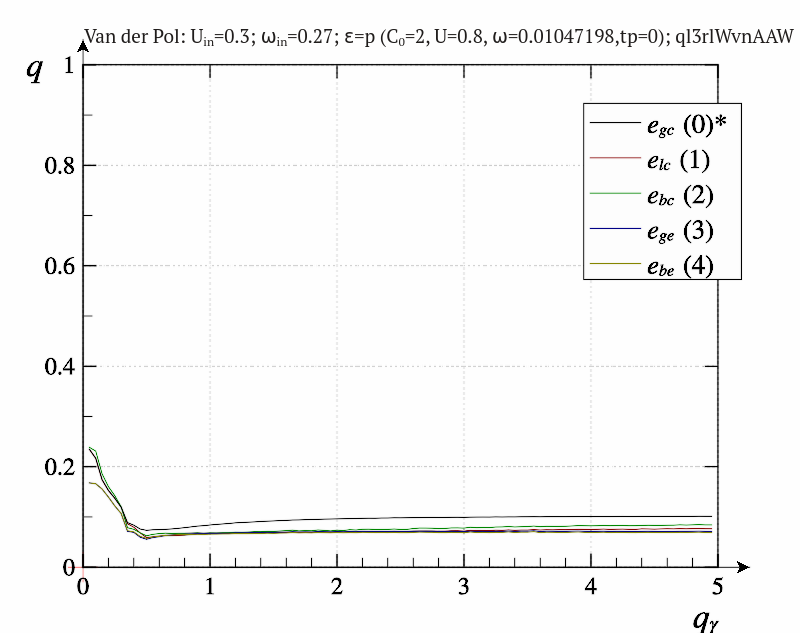
\includegraphics[width=0.49\textwidth]{p/cha/vdp/vdp_id-p_q_gamma_sin.png}
\end{center}
  \caption{Зависимости $\bar{e}(q_\gamma)$ для системы Ван-дер-Поля}
\label{atu:f:vdp_e_q_gamma}
\end{figure}

Используемая группа методов ``ql3rlWvnAAW'' характеризуется
работоспособностью для широкого диапазона величины $q_\gamma$,
за исключением области избыточной чувствительности,
к которой поиск всё же возможен, но
его диапазон ограничивается малой окрестностью агентов.
Представленные графики полностью это подтверждают.
Применение различных методов определения $p_\mathrm{id}$
по разному себя проявляет в области заниженной чувствительности,
но это различие мало.


Зависимости $\bar{e}(v_f)$ полученные при идентификации системы Ван-дер-Поля
(рис.~\ref{atu:f:vdp_e_v_f}), демонстрируют
существенную разницу при различных способах
задания нестационарности  параметра.

\begin{figure}[ht!]
\begin{center}
  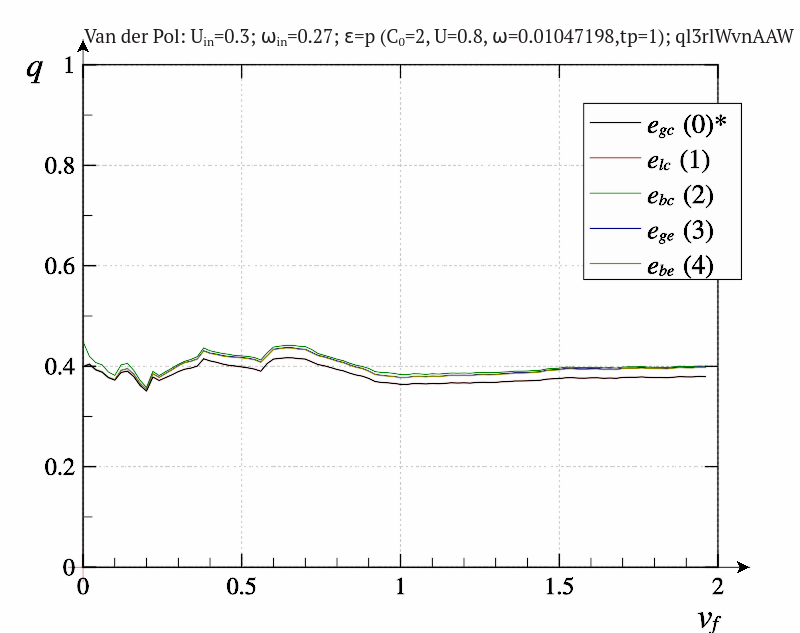
\includegraphics[width=0.49\textwidth]{p/cha/vdp/vdp_id-p_v_f_sign.png}
  \hfill
  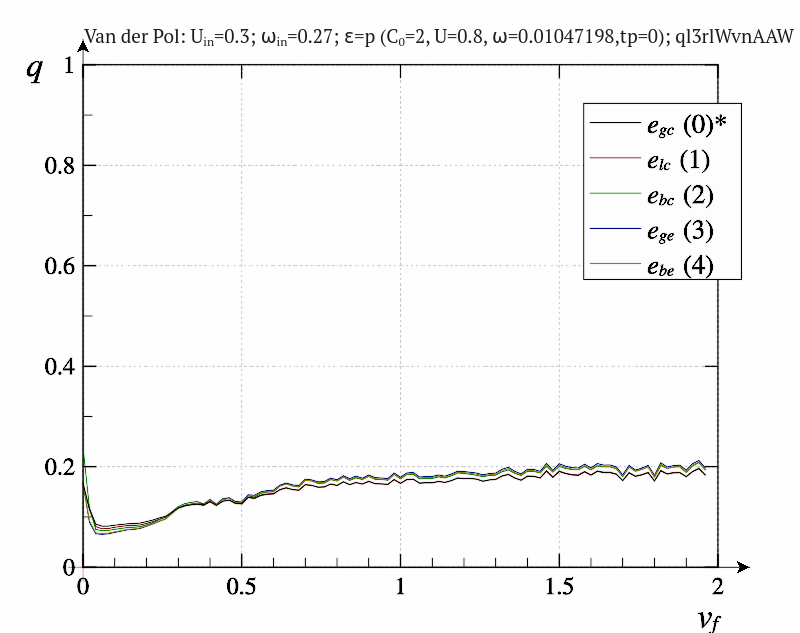
\includegraphics[width=0.49\textwidth]{p/cha/vdp/vdp_id-p_v_f_sin.png}
\end{center}
  \caption{Зависимости $\bar{e}(v_f)$ для системы Ван-дер-Поля}
\label{atu:f:vdp_e_v_f}
\end{figure}

Если в динамике идентифицируемого параметра нет
резких изменений (правый график), то
зависимости имеют классический вид,
существует такое значение $v_f$, при котором наблюдается
минимум ошибки. В том же случае, когда зависимость представляет собой
зависимость с разрывами (\ref{atu:eq:po_t_sign}),
то зависимость получается слабая и неоднозначная.
Это связано с тем, что перестройка положений агентов
хоть и происходит, но не приводит к уменьшению ошибки
ввиду того, что время реакции критерия становится одного порядка
с временем реакции на изменение параметра.


Влияние коэффициента $k_e$ (рис.~\ref{atu:f:vdp_e_k_e})
для данной системы также существенно зависит от динамики
параметра, и по той же причине.
Если динамика параметра задана как (\ref{atu:eq:po_t_sin}),
то существует экстремум, соответствующий оптимальному распределению агентов.
При скачкообразных изменениях параметра экстремум практически незаметен
на общем фоне.

\begin{figure}[ht!]
\begin{center}
  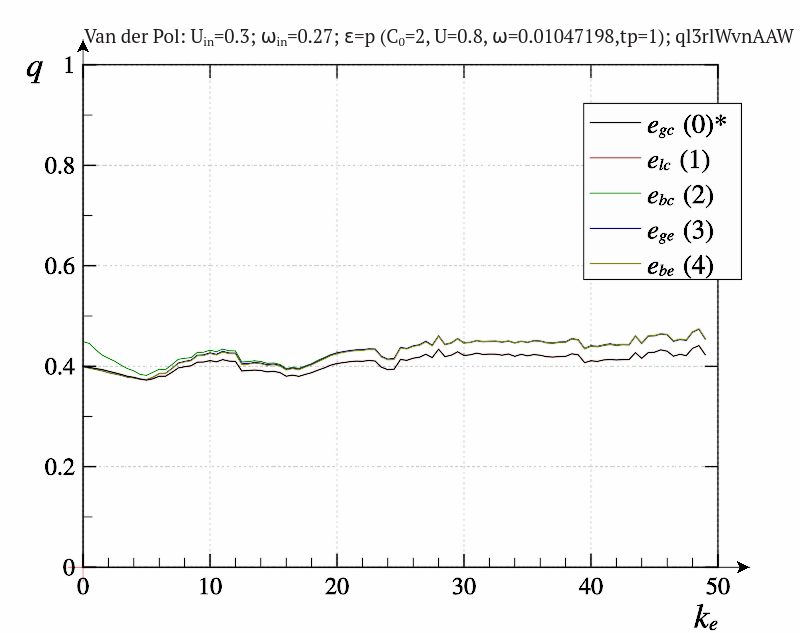
\includegraphics[width=0.49\textwidth]{p/cha/vdp/vdp_id-p_k_e_sign.png}
  \hfill
  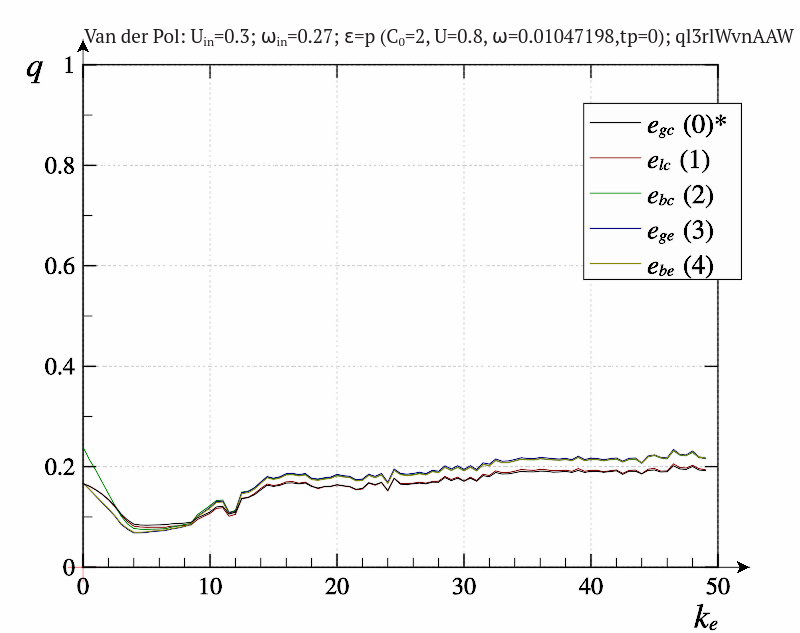
\includegraphics[width=0.49\textwidth]{p/cha/vdp/vdp_id-p_k_e_sin.png}
\end{center}
  \caption{Зависимости $\bar{e}(k_e)$ для системы Ван-дер-Поля}
\label{atu:f:vdp_e_k_e}
\end{figure}

Влияние параметра $k_{nl}$ (рис.~\ref{atu:f:vdp_e_k_nl})
отображает свойства множества агентов как ансамбля.
В отличие от двух предыдущих зависимостей,
минимум ошибки идентификации наблюдается для двух
способов определения динамики параметров, то есть
корректное взаимодействие между агентами необходимо
для получения результата даже в тех случаях,
когда собственно перемещение агентов не оправдано.

\begin{figure}[ht!]
\begin{center}
  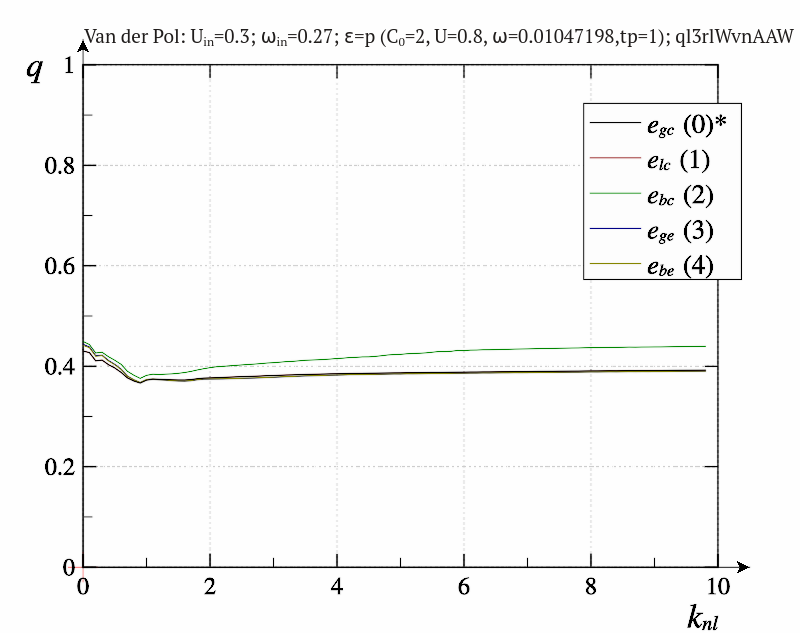
\includegraphics[width=0.49\textwidth]{p/cha/vdp/vdp_id-p_k_nl_sign.png}
  \hfill
  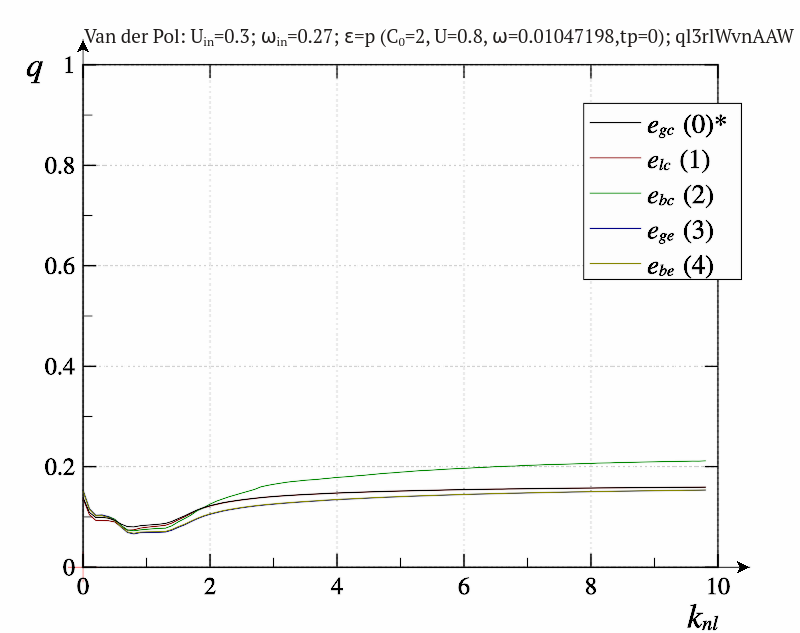
\includegraphics[width=0.49\textwidth]{p/cha/vdp/vdp_id-p_k_nl_sin.png}
\end{center}
  \caption{Зависимости $\bar{e}(k_{nl})$ для системы Ван-дер-Поля}
\label{atu:f:vdp_e_k_nl}
\end{figure}

Как и в предыдущем случае,
искусственные ограничения на перемещения агентов
практически нивелирует влияние коэффициента $k_{cl}$ (рис.~\ref{atu:f:vdp_e_k_cl}).
В этих условиях силу $f_c$ имеет смысл вообще не определять.

\begin{figure}[ht!]
\begin{center}
  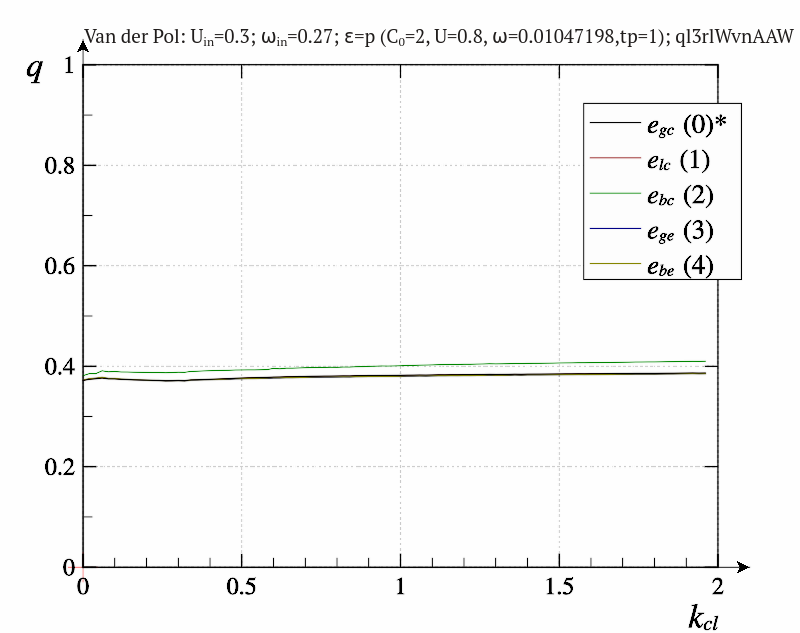
\includegraphics[width=0.49\textwidth]{p/cha/vdp/vdp_id-p_k_cl_sign.png}
  \hfill
  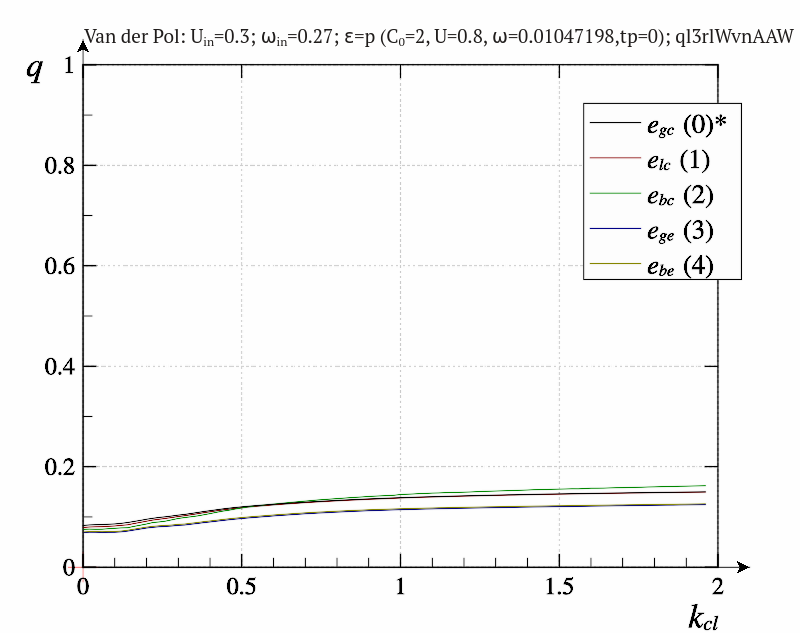
\includegraphics[width=0.49\textwidth]{p/cha/vdp/vdp_id-p_k_cl_sin.png}
\end{center}
  \caption{Зависимости $\bar{e}(k_{cl})$ для системы Ван-дер-Поля}
\label{atu:f:vdp_e_k_cl}
\end{figure}

На  рис.~\ref{atu:f:vdp_e_varepsilon_2} представлена зависимость ошибки идентификации
от величины самого параметра $\varepsilon$ в условиях,
когда постоянно чередуются хаотические и сложно-периодические режимы.
В этих условиях ошибка идентификации возрастает,
но сама система идентификации остаётся работоспособной.


\begin{figure}[ht!]
\begin{center}
  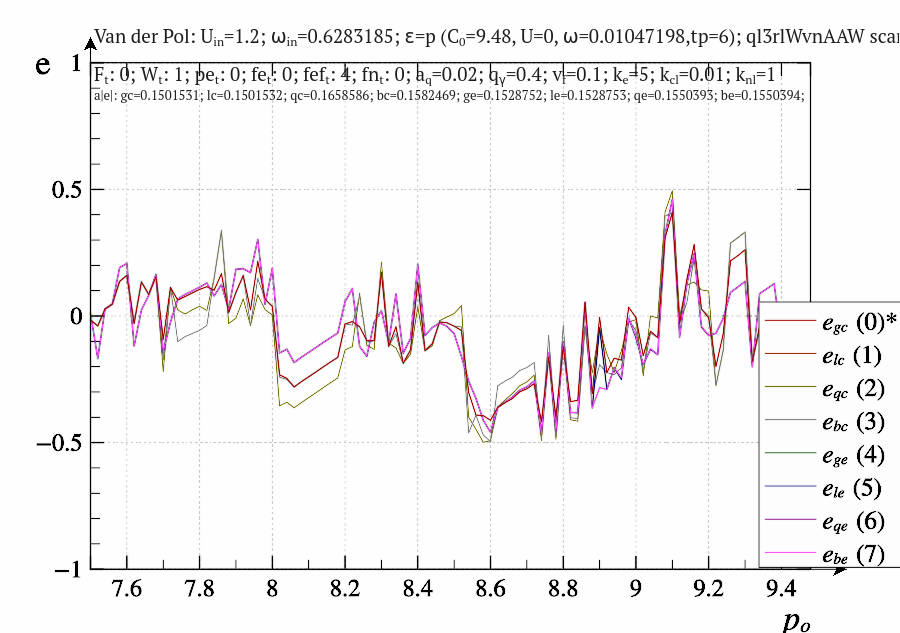
\includegraphics[width=0.60\textwidth]{p/cha/vdp/vdp_id2-p_p_e_ql3rlWvnAAW_scan.png}
\end{center}
  \caption{Зависимости $\bar{e}(\varepsilon)$ для системы Ван-дер-Поля в условиях чередования режимов колебаний}
\label{atu:f:vdp_e_varepsilon_2}
\end{figure}

% }}}2

\subsection{Выводы}  % {{{2

Результаты моделирования
процессов идентификации параметра ``$\varepsilon$''
системы Ван-дер-Поля
позволяют в сделать следующие выводы:

\begin{itemize}

  \item
    Наибольший диапазон примерности для этой системы
    демонстрирует критерий $q_T$ с последующим усреднением.

  \item
    Не обнаружено критерия, который бы был работоспособен во всей
    области определения параметров, в связи с разнообразием динамики,
    которую проявляет система.

  \item
    Группа методов ql3rlWvnAAW показала свою хорошую работоспособность,
    даже в условиях чередования режимов колебаний.

  \item
    Параметры самой системы идентификации могут изменяться в достаточно широких
    пределах без существенного увеличения ошибки идентификации.

\end{itemize}

% }}}2



% }}}1

% vim: fdm=marker foldlevel=1 foldignore="%#" fdc=4 ft=tex
